\documentclass[aspectratio=169,10pt]{beamer}

\usetheme{Madrid}
\usecolortheme{default}
\usepackage{amsmath}
\usepackage{bm}
\usepackage{booktabs}
\usepackage{graphicx}
\usepackage{hyperref}

\graphicspath{{../results/figures/}}

\definecolor{iitblue}{RGB}{24,67,105}
\definecolor{accentgreen}{RGB}{18,130,118}
\definecolor{warmgray}{RGB}{92,96,104}
\definecolor{lightband}{RGB}{244,247,250}

\setbeamercolor{palette primary}{bg=iitblue,fg=white}
\setbeamercolor{palette secondary}{bg=accentgreen,fg=white}
\setbeamercolor{frametitle}{bg=iitblue,fg=white}
\setbeamercolor{title}{fg=iitblue}
\setbeamercolor{block title}{bg=iitblue,fg=white}
\setbeamercolor{block body}{bg=lightband,fg=black}
\setbeamertemplate{navigation symbols}{}
\setbeamertemplate{footline}[frame number]

\newcommand{\smallgap}{\vspace{0.35em}}
\newcommand{\keyclaim}[1]{\begin{block}{Key message}#1\end{block}}

\title[Fuzzy-Supervised Residual RL]{Fuzzy-Supervised Residual Reinforcement Learning\\for Robust Robot Manipulator Tracking}
\subtitle{From term-paper concept to reproducible robustness benchmark}
\author[Vedant Meshram]{Vedant Meshram}
\institute[IIT Kharagpur]{Department of Mechanical Engineering\\Indian Institute of Technology Kharagpur}
\date{\today}

\begin{document}

\begin{frame}
  \titlepage
\end{frame}

\begin{frame}{Why This Problem Matters}
  \begin{columns}[T,onlytextwidth]
    \begin{column}{0.52\textwidth}
      Industrial manipulators are rarely operated under one fixed model.
      \smallgap
      \begin{itemize}
        \item Payload changes alter inertia and gravity loading.
        \item Friction drift and disturbances break fixed-gain assumptions.
        \item Direct torque-space RL can fail during exploration.
      \end{itemize}
    \end{column}
    \begin{column}{0.42\textwidth}
      \begin{block}{Research question}
        Can an interpretable fuzzy supervisor make residual RL safer and more useful under plant mismatch?
      \end{block}
    \end{column}
  \end{columns}
  \vfill
  \keyclaim{The goal is not to replace classical control everywhere. The goal is to add adaptive residual authority only where mismatch makes it valuable.}
\end{frame}

\begin{frame}{Positioning the Idea}
  \begin{columns}[T,onlytextwidth]
    \begin{column}{0.48\textwidth}
      \begin{block}{What fuzzy control gives}
        \begin{itemize}
          \item Linguistic, interpretable rule base.
          \item Immediate stabilizing baseline.
          \item Low sample cost and predictable response.
        \end{itemize}
      \end{block}
    \end{column}
    \begin{column}{0.48\textwidth}
      \begin{block}{What residual RL gives}
        \begin{itemize}
          \item Learned compensation for unmodeled shifts.
          \item Continuous torque correction.
          \item Adaptation through reward feedback.
        \end{itemize}
      \end{block}
    \end{column}
  \end{columns}
  \vfill
  \begin{center}
    \Large $\bm{\tau}=\bm{\tau}_{\mathrm{fuzzy}}+g(\bm{e},\dot{\bm{e}},\xi)\bm{\tau}_{\mathrm{RL}}$
  \end{center}
\end{frame}

\begin{frame}{Controller Architecture}
  \begin{columns}[T,onlytextwidth]
    \begin{column}{0.54\textwidth}
      \begin{block}{Hybrid control law}
        \[
          \bm{\tau}=\bm{\tau}_{\mathrm{fuzzy}}+g(\bm{e},\dot{\bm{e}},\xi)\bm{\tau}_{\mathrm{RL}},
          \quad \|\bm{\tau}_{\mathrm{RL}}\|_\infty \leq \bar{\tau}_r .
        \]
      \end{block}
      \begin{itemize}
        \item Mamdani fuzzy supervisor uses $e$ and $\dot e$.
        \item TD3 or SAC learns bounded residual torque.
        \item Gate $g\in[0,1]$ suppresses residual action during nominal tracking.
      \end{itemize}
    \end{column}
    \begin{column}{0.40\textwidth}
      \begin{block}{Uncertainty gate}
        \[
        \begin{aligned}
        g=\operatorname{clip}\bigg(&
        \left(\frac{\|\bm e\|}{\epsilon_g}\right)^2
        +0.2\left(\frac{\xi}{\epsilon_g}\right)^2\\
        &+0.05\eta,0,1\bigg).
        \end{aligned}
        \]
        \small $\xi$ is persistent tracking error; $\eta$ is normalized velocity-error activity.
      \end{block}
    \end{column}
  \end{columns}
\end{frame}

\begin{frame}{What Changed From the Original Claim}
  \begin{block}{Old inflated claim}
    Hybrid Fuzzy-TD3 is universally superior for trajectory tracking.
  \end{block}
  \begin{block}{Revised defensible claim}
    Fuzzy-supervised residual RL is a robustness layer: it improves shifted-plant tracking and avoids direct-RL failures, while uncertainty gating is needed to preserve nominal performance.
  \end{block}
  \begin{itemize}
    \item No DQN comparison is claimed.
    \item Comparisons are against PID, fuzzy-only, model-based baselines, TD3, SAC, DDPG, residual TD3, and residual SAC.
    \item 6-DOF validation is stated as required future work, not as completed evidence.
  \end{itemize}
\end{frame}

\begin{frame}{Experimental Protocol}
  \begin{columns}[T,onlytextwidth]
    \begin{column}{0.50\textwidth}
      \begin{block}{Benchmark}
        \begin{itemize}
          \item Two-link rigid-body manipulator.
          \item Step size: 20 ms; horizon: 6 s.
          \item Torque saturation: 35 Nm.
          \item Disturbances begin at 2.5 s.
        \end{itemize}
      \end{block}
    \end{column}
    \begin{column}{0.46\textwidth}
      \begin{block}{Scenarios}
        \begin{itemize}
          \item Nominal plant.
          \item Payload doubled, friction increased.
          \item Severe shift: payload tripled, stronger friction and sinusoidal disturbance.
        \end{itemize}
      \end{block}
    \end{column}
  \end{columns}
  \vfill
  Five seeds, 12000 training steps per learned controller, and 20 evaluation rollouts per controller per scenario.
\end{frame}

\begin{frame}{Baselines and Metrics}
  \begin{columns}[T,onlytextwidth]
    \begin{column}{0.53\textwidth}
      \begin{block}{Baselines}
        \begin{itemize}
          \item PID and robust PID/sliding-mode term.
          \item Computed torque and adaptive computed torque.
          \item Fuzzy-only and tuned fuzzy.
          \item Direct TD3, SAC, DDPG.
          \item Residual TD3, residual SAC, gated Fuzzy-TD3.
        \end{itemize}
      \end{block}
    \end{column}
    \begin{column}{0.43\textwidth}
      \begin{block}{Metrics}
        \begin{itemize}
          \item Joint RMSE.
          \item Failure-penalized RMSE.
          \item Safety-violation rate.
          \item Torque smoothness RMS.
          \item Completion rate.
        \end{itemize}
      \end{block}
    \end{column}
  \end{columns}
  \vfill
  \small Failure-penalized RMSE prevents early-failing direct-RL rollouts from looking deceptively good.
\end{frame}

\begin{frame}{Main Result: Shifted-Plant Robustness}
  \begin{columns}[T,onlytextwidth]
    \begin{column}{0.57\textwidth}
      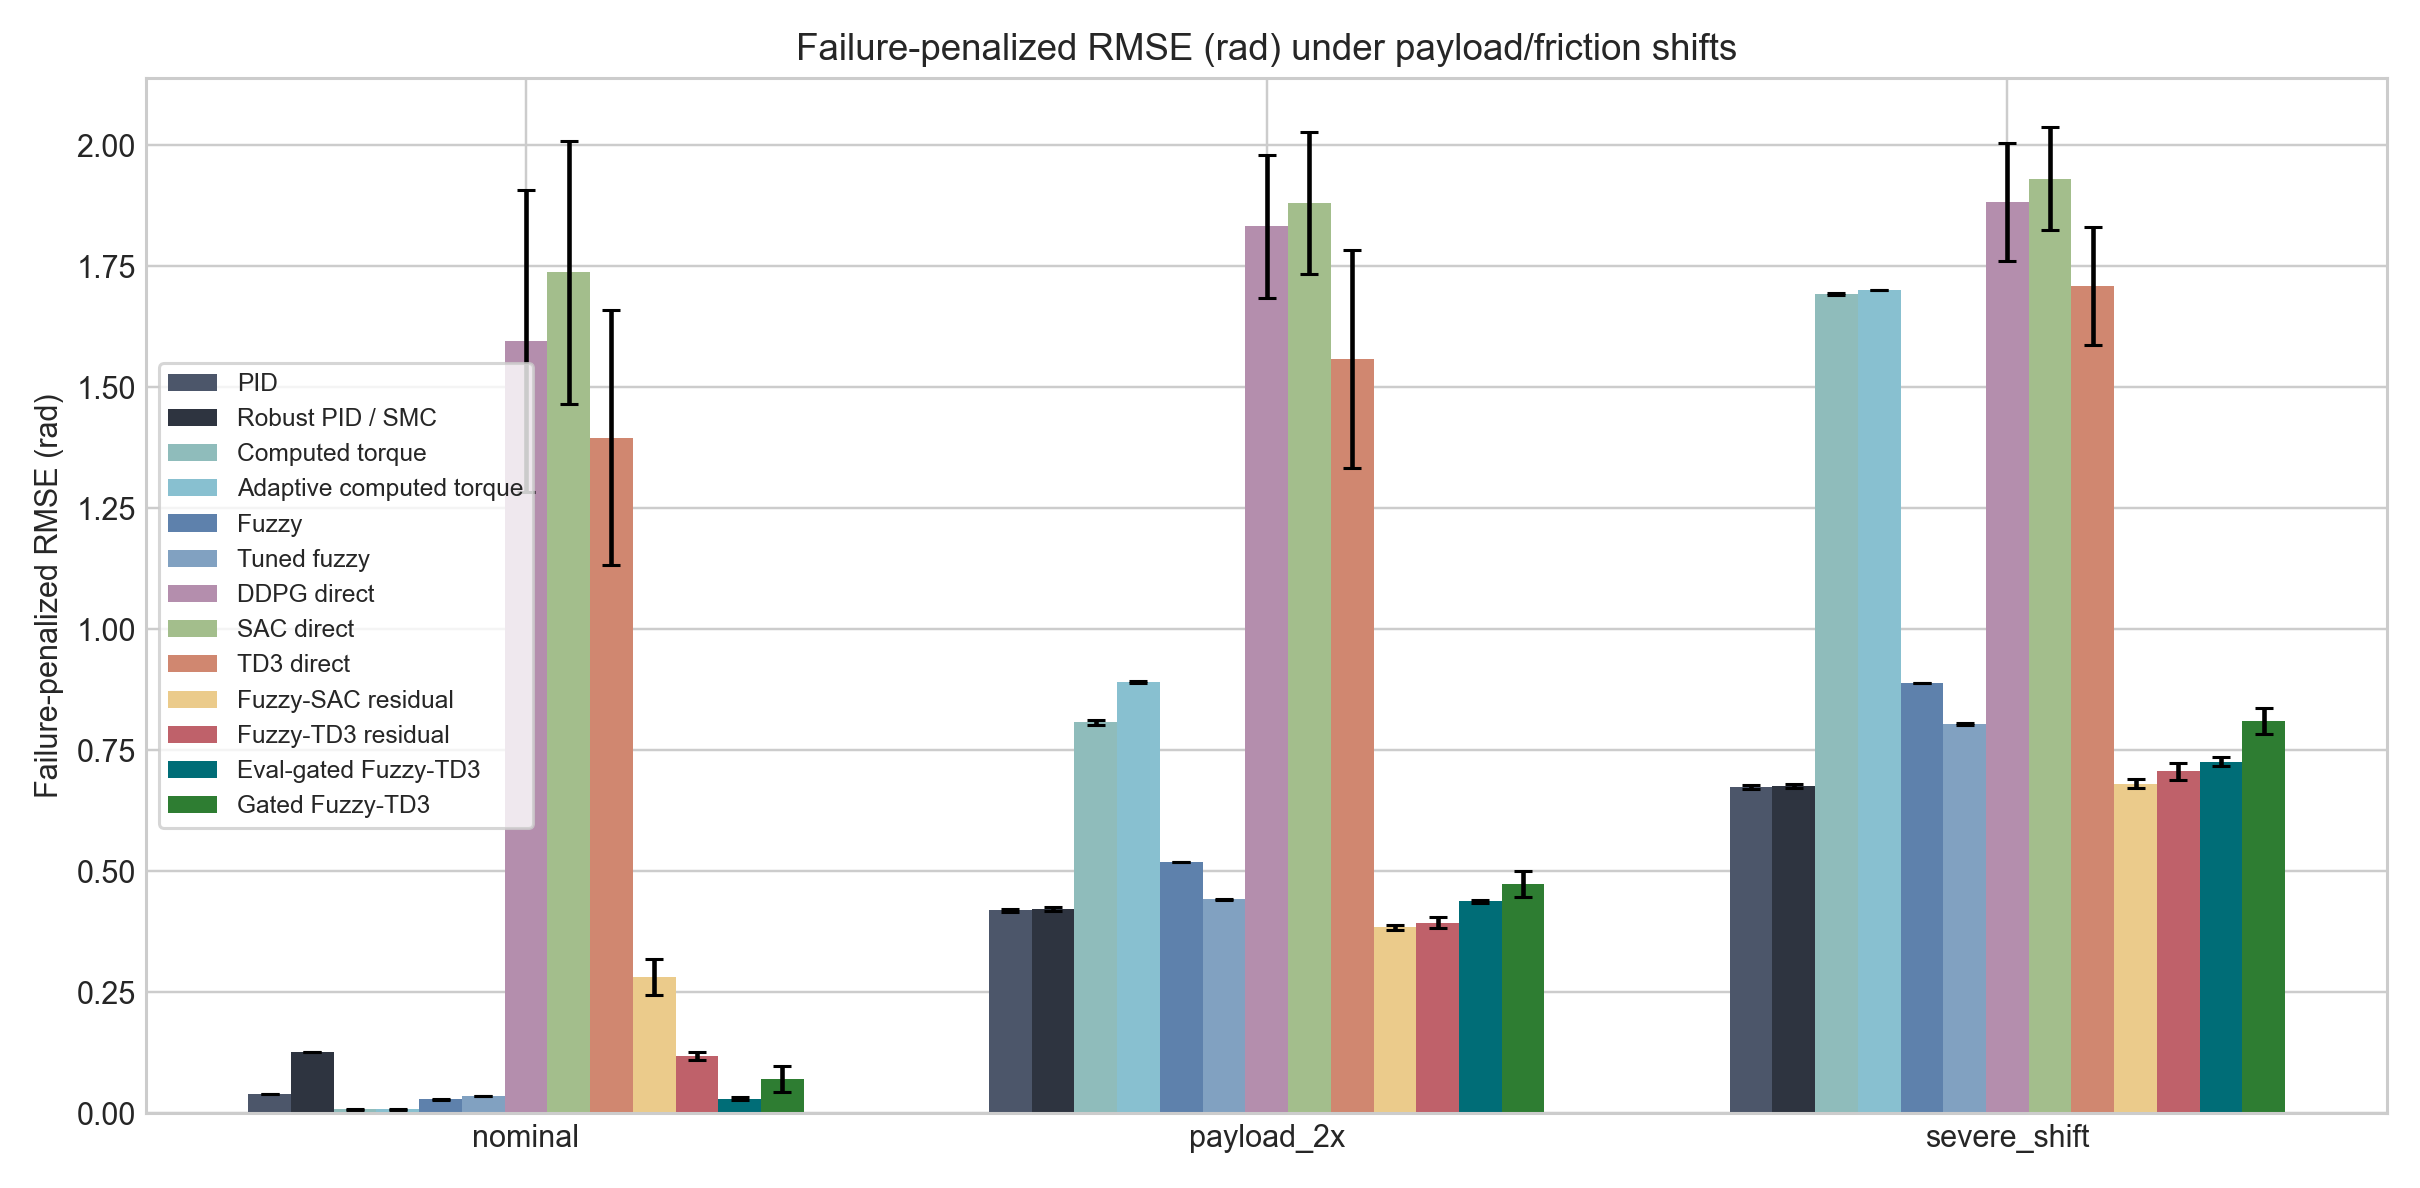
\includegraphics[width=\linewidth]{penalized_rmse_by_scenario.png}
    \end{column}
    \begin{column}{0.39\textwidth}
      \begin{block}{Interpretation}
        \begin{itemize}
          \item Model-based control dominates nominal tracking.
          \item Direct RL fails frequently.
          \item Residual SAC and residual TD3 improve under payload/friction shifts.
          \item Gating nearly fixes nominal degradation.
        \end{itemize}
      \end{block}
    \end{column}
  \end{columns}
\end{frame}

\begin{frame}{Numerical Takeaways}
  \begin{table}
    \centering
    \small
    \begin{tabular}{llccc}
      \toprule
      Scenario & Controller & Penalized RMSE & Safety & Completion \\
      \midrule
      Nominal & Fuzzy & 0.0284 & 0.000 & 1.00 \\
      Nominal & Eval-gated Fuzzy-TD3 & 0.0299 & 0.000 & 1.00 \\
      Payload-2x & Fuzzy-SAC residual & 0.3839 & 0.172 & 1.00 \\
      Payload-2x & Fuzzy-TD3 residual & 0.3936 & 0.175 & 1.00 \\
      Payload-2x & PID & 0.4190 & 0.187 & 1.00 \\
      Severe shift & PID & 0.6739 & 0.273 & 1.00 \\
      Severe shift & Fuzzy-SAC residual & 0.6804 & 0.266 & 1.00 \\
      Severe shift & Fuzzy-TD3 residual & 0.7065 & 0.272 & 1.00 \\
      \bottomrule
    \end{tabular}
  \end{table}
  \vfill
  \keyclaim{Residual SAC is the strongest learned controller; residual TD3 remains competitive; both avoid the failure behavior of direct RL.}
\end{frame}

\begin{frame}{Safety: Direct RL vs Supervised Residual RL}
  \begin{columns}[T,onlytextwidth]
    \begin{column}{0.56\textwidth}
      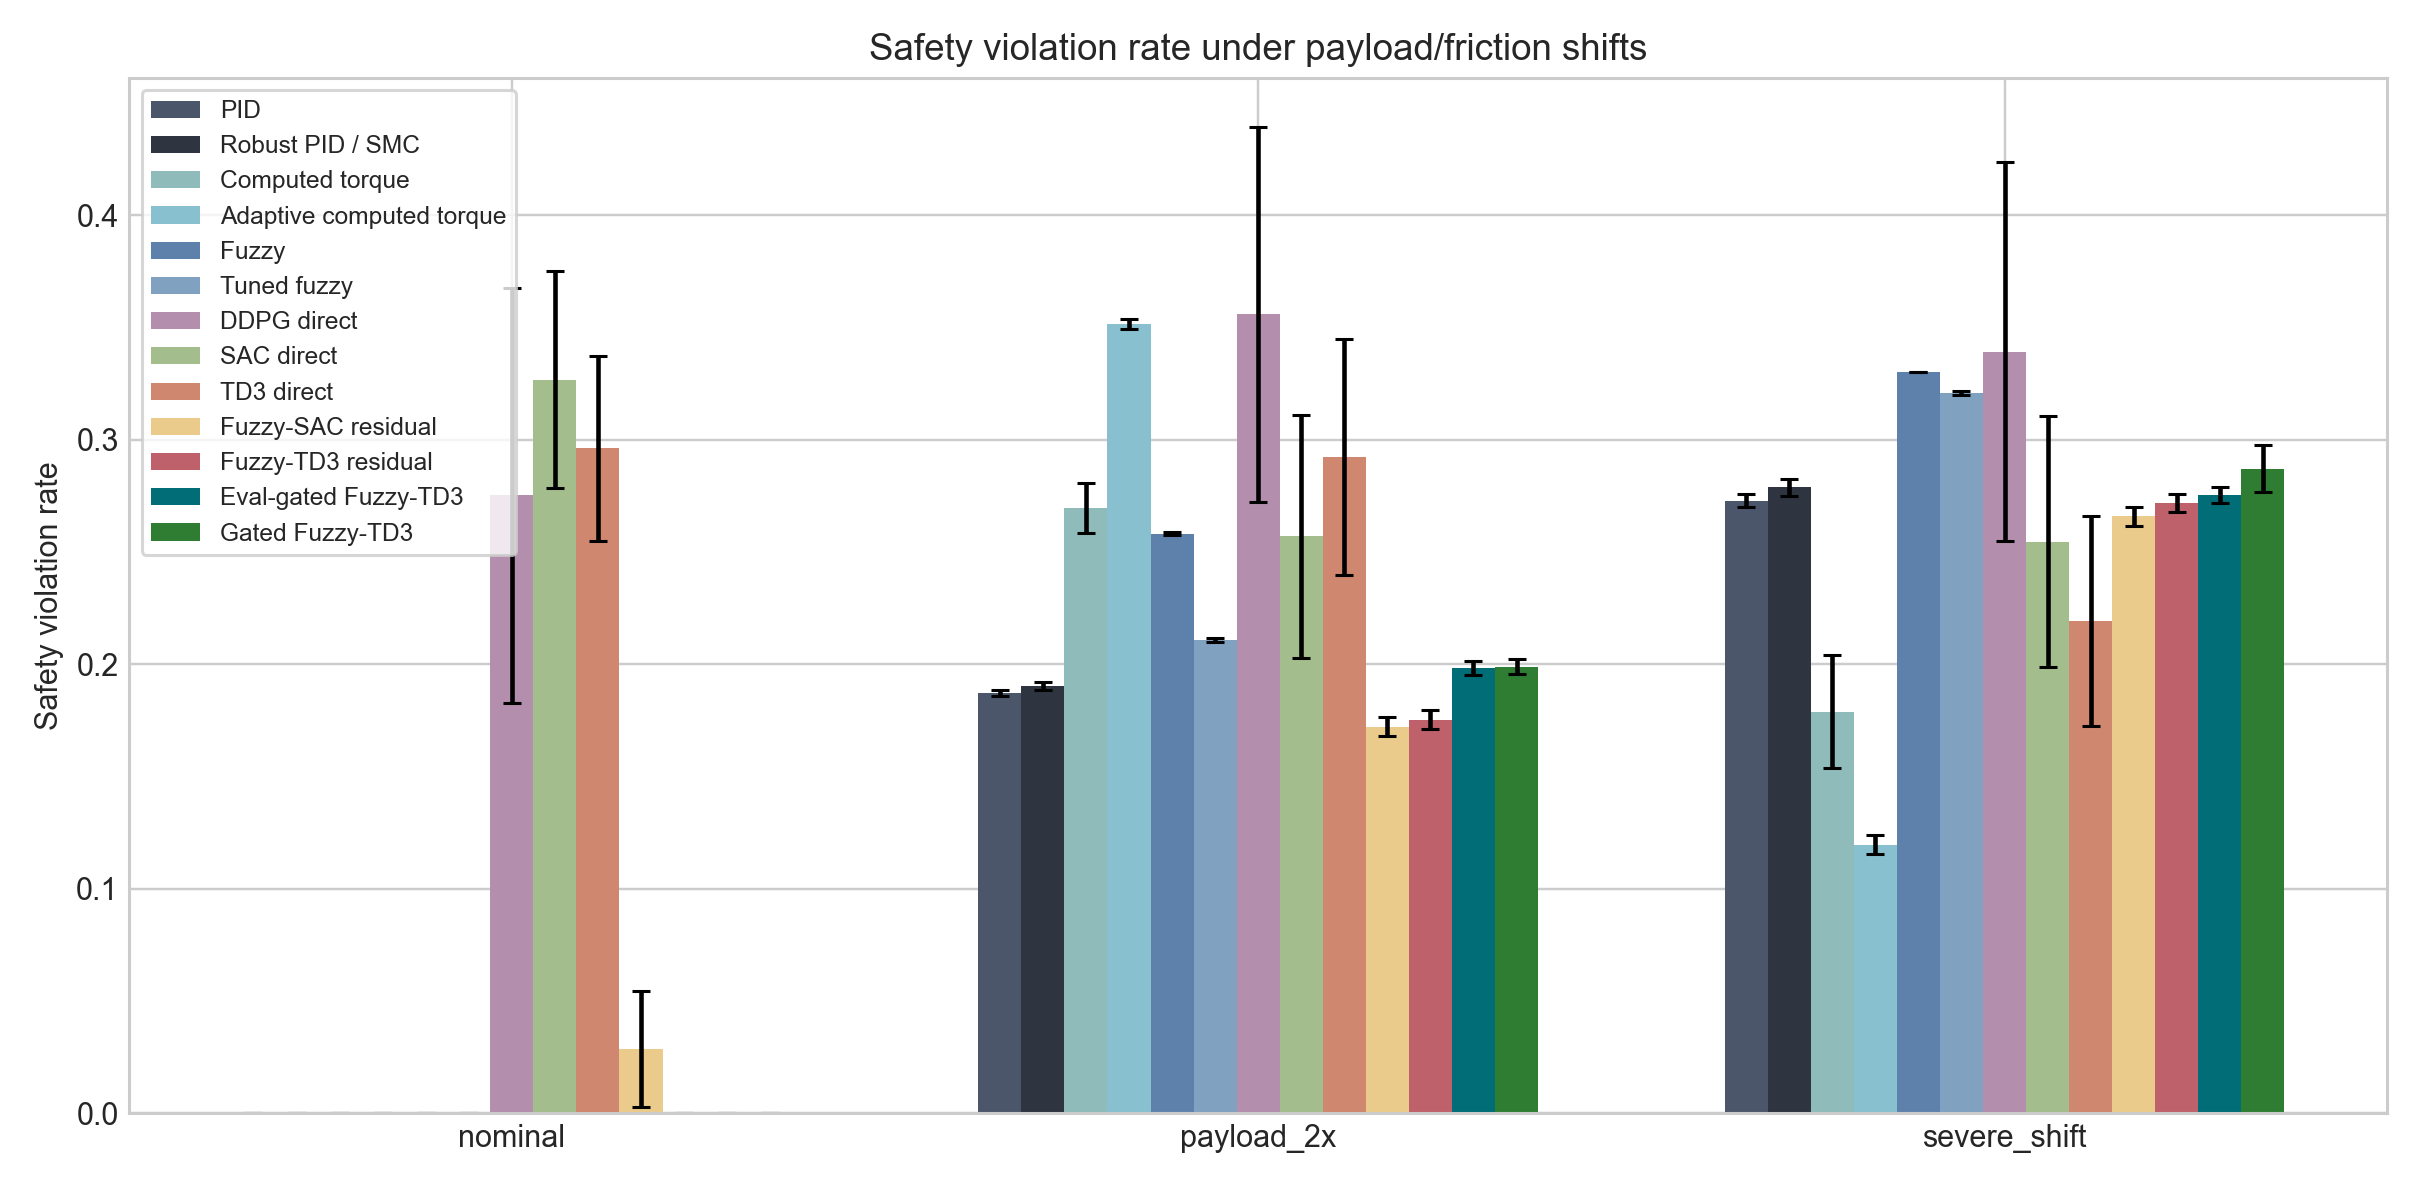
\includegraphics[width=\linewidth]{safety_by_scenario.png}
    \end{column}
    \begin{column}{0.40\textwidth}
      \begin{block}{What the plot shows}
        \begin{itemize}
          \item Direct TD3/SAC/DDPG often violate safety thresholds.
          \item Residual policies inherit fuzzy baseline structure.
          \item Bounded residual authority limits worst-case exploration.
        \end{itemize}
      \end{block}
      \smallgap
      \small This is empirical safety, not a formal proof.
    \end{column}
  \end{columns}
\end{frame}

\begin{frame}{Torque Smoothness}
  \begin{columns}[T,onlytextwidth]
    \begin{column}{0.58\textwidth}
      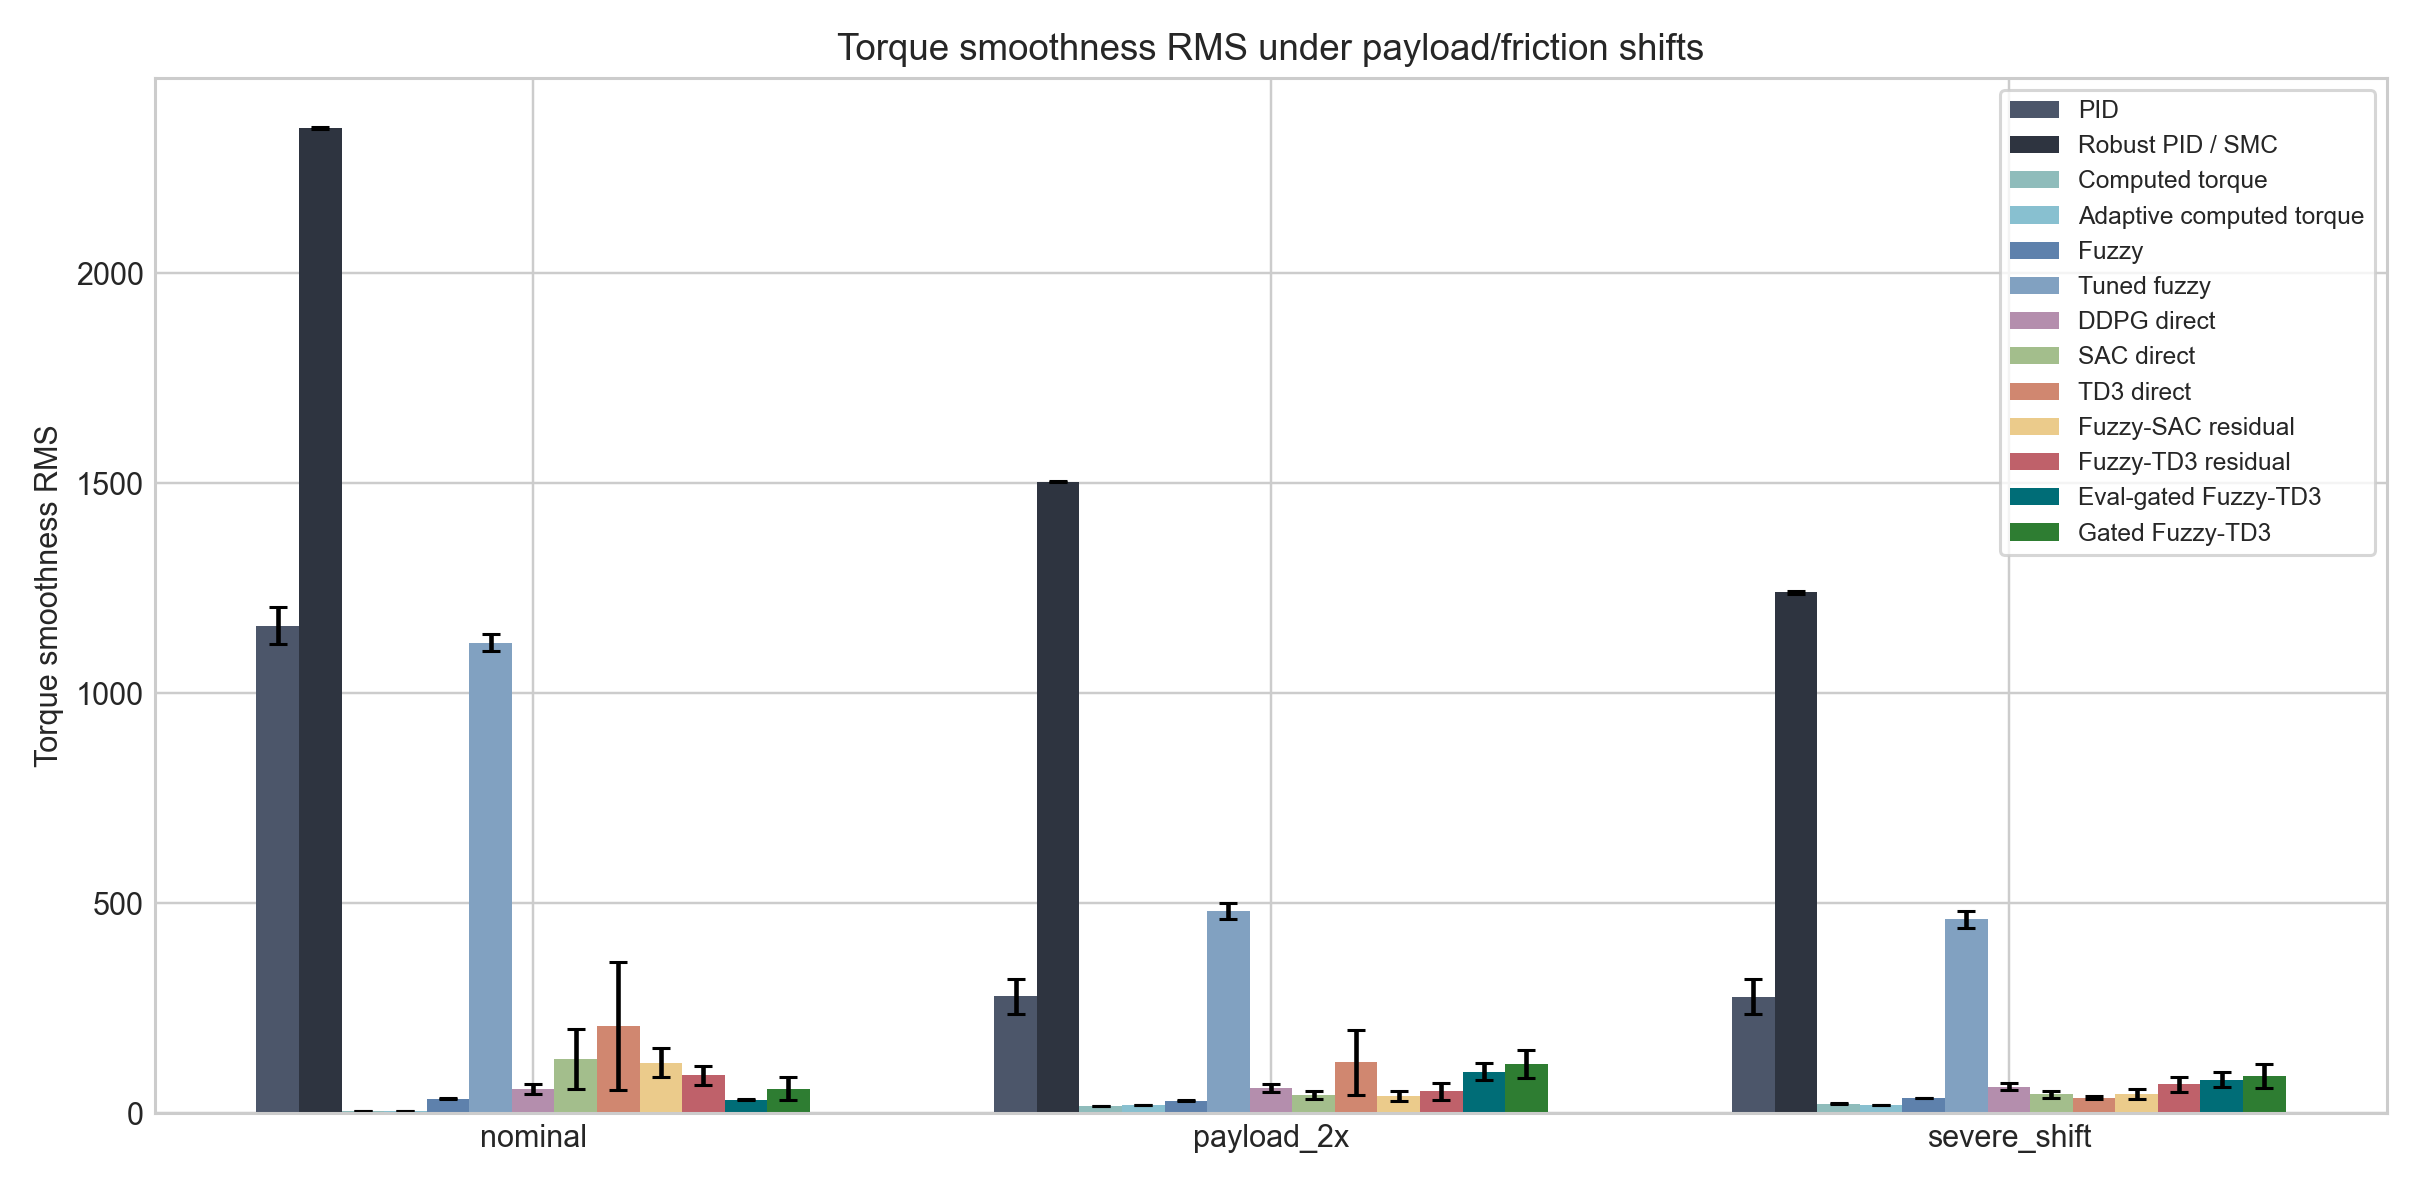
\includegraphics[width=\linewidth]{torque_smoothness_by_scenario.png}
    \end{column}
    \begin{column}{0.38\textwidth}
      \begin{block}{Why this matters}
        \begin{itemize}
          \item PID and robust PID can track shifts but may be torque-rough.
          \item Residual SAC is close to PID tracking in severe shift with much smoother torque.
          \item Smoothness is important for actuator wear and deployment credibility.
        \end{itemize}
      \end{block}
    \end{column}
  \end{columns}
\end{frame}

\begin{frame}{Gating Fixes the Main Weakness}
  \begin{columns}[T,onlytextwidth]
    \begin{column}{0.48\textwidth}
      \begin{block}{Problem}
        Always-active residual TD3 hurts nominal tracking:
        \[
          0.1184\ \mathrm{rad}
        \]
        versus fuzzy-only:
        \[
          0.0284\ \mathrm{rad}.
        \]
      \end{block}
    \end{column}
    \begin{column}{0.48\textwidth}
      \begin{block}{Gated result}
        Evaluation-gated Fuzzy-TD3:
        \[
          0.0299\ \mathrm{rad}
        \]
        with mean nominal gate:
        \[
          g=0.034.
        \]
      \end{block}
    \end{column}
  \end{columns}
  \vfill
  \keyclaim{The publishable direction is uncertainty-gated residual learning, not always-on residual action.}
\end{frame}

\begin{frame}{Ablation: Residual Authority}
  \begin{columns}[T,onlytextwidth]
    \begin{column}{0.56\textwidth}
      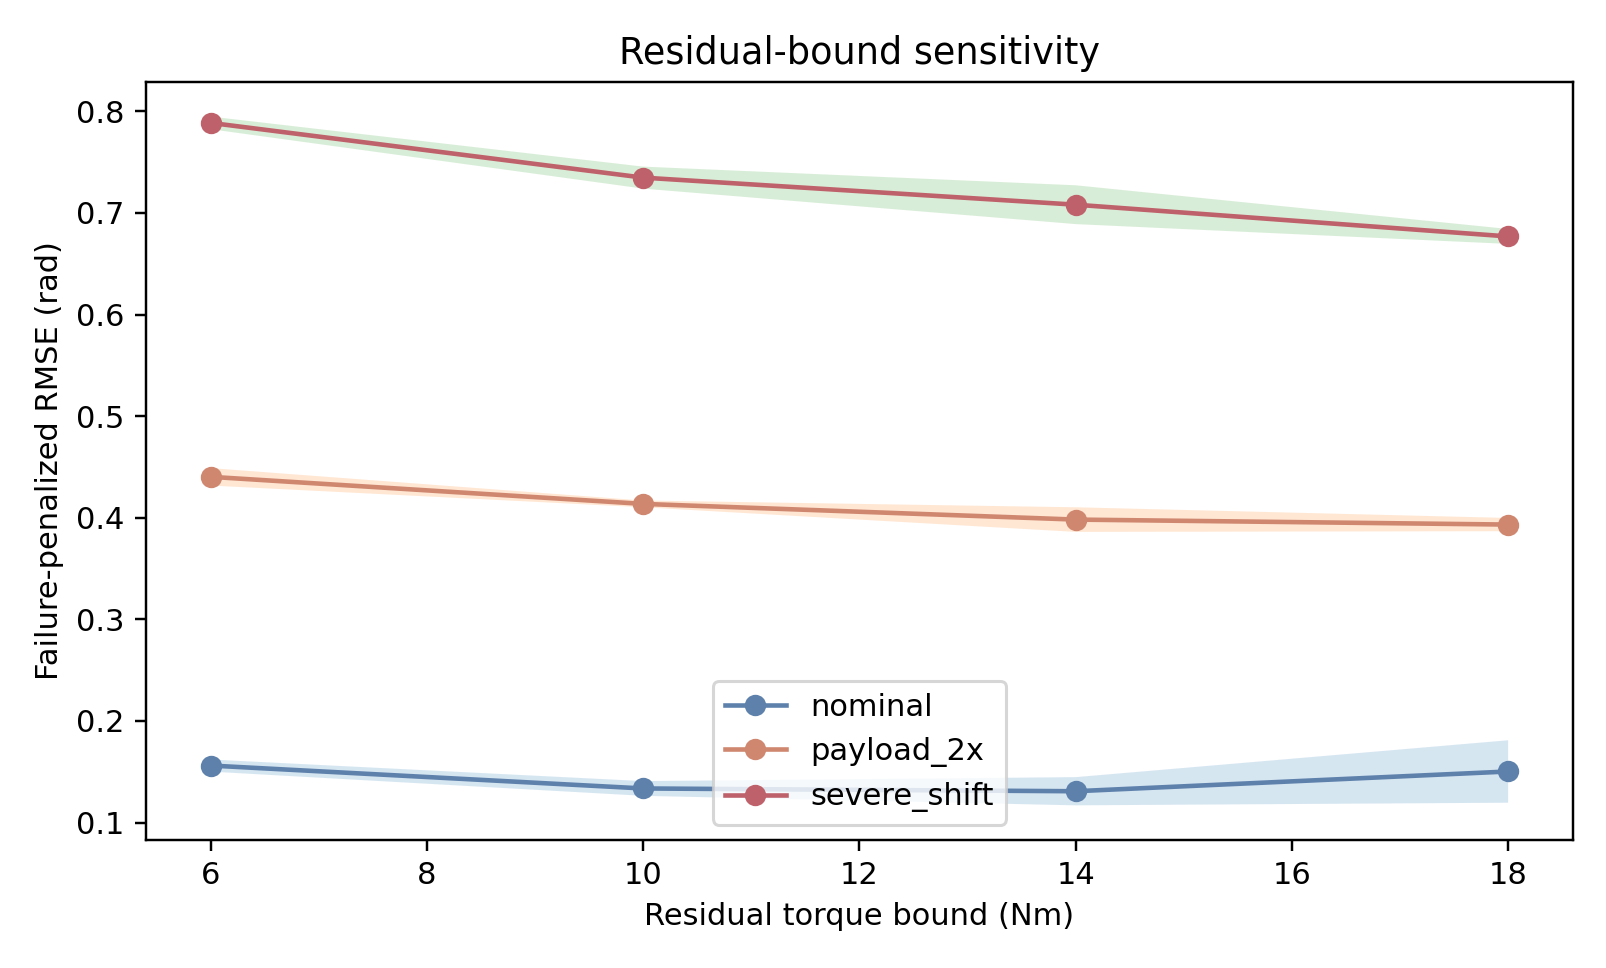
\includegraphics[width=\linewidth]{ablation_residual_bound_rmse.png}
    \end{column}
    \begin{column}{0.40\textwidth}
      \begin{block}{Trade-off}
        \begin{itemize}
          \item Larger residual bounds improve shifted-plant tracking.
          \item Every nonzero bound hurts nominal tracking.
          \item This directly motivates uncertainty gating.
        \end{itemize}
      \end{block}
    \end{column}
  \end{columns}
\end{frame}

\begin{frame}{Ablation Table}
  \begin{table}
    \centering
    \small
    \begin{tabular}{lccccc}
      \toprule
      Scenario & 0 Nm & 6 Nm & 10 Nm & 14 Nm & 18 Nm \\
      \midrule
      Nominal & 0.0292 & 0.1561 & 0.1335 & 0.1308 & 0.1502 \\
      Payload-2x & 0.5192 & 0.4403 & 0.4136 & 0.3982 & 0.3933 \\
      Severe shift & 0.8891 & 0.7887 & 0.7348 & 0.7081 & 0.6769 \\
      \bottomrule
    \end{tabular}
  \end{table}
  \vfill
  \small Values are failure-penalized RMSE means over five seeds and twenty evaluation rollouts per setting.
\end{frame}

\begin{frame}{Representative Severe-Shift Rollout}
  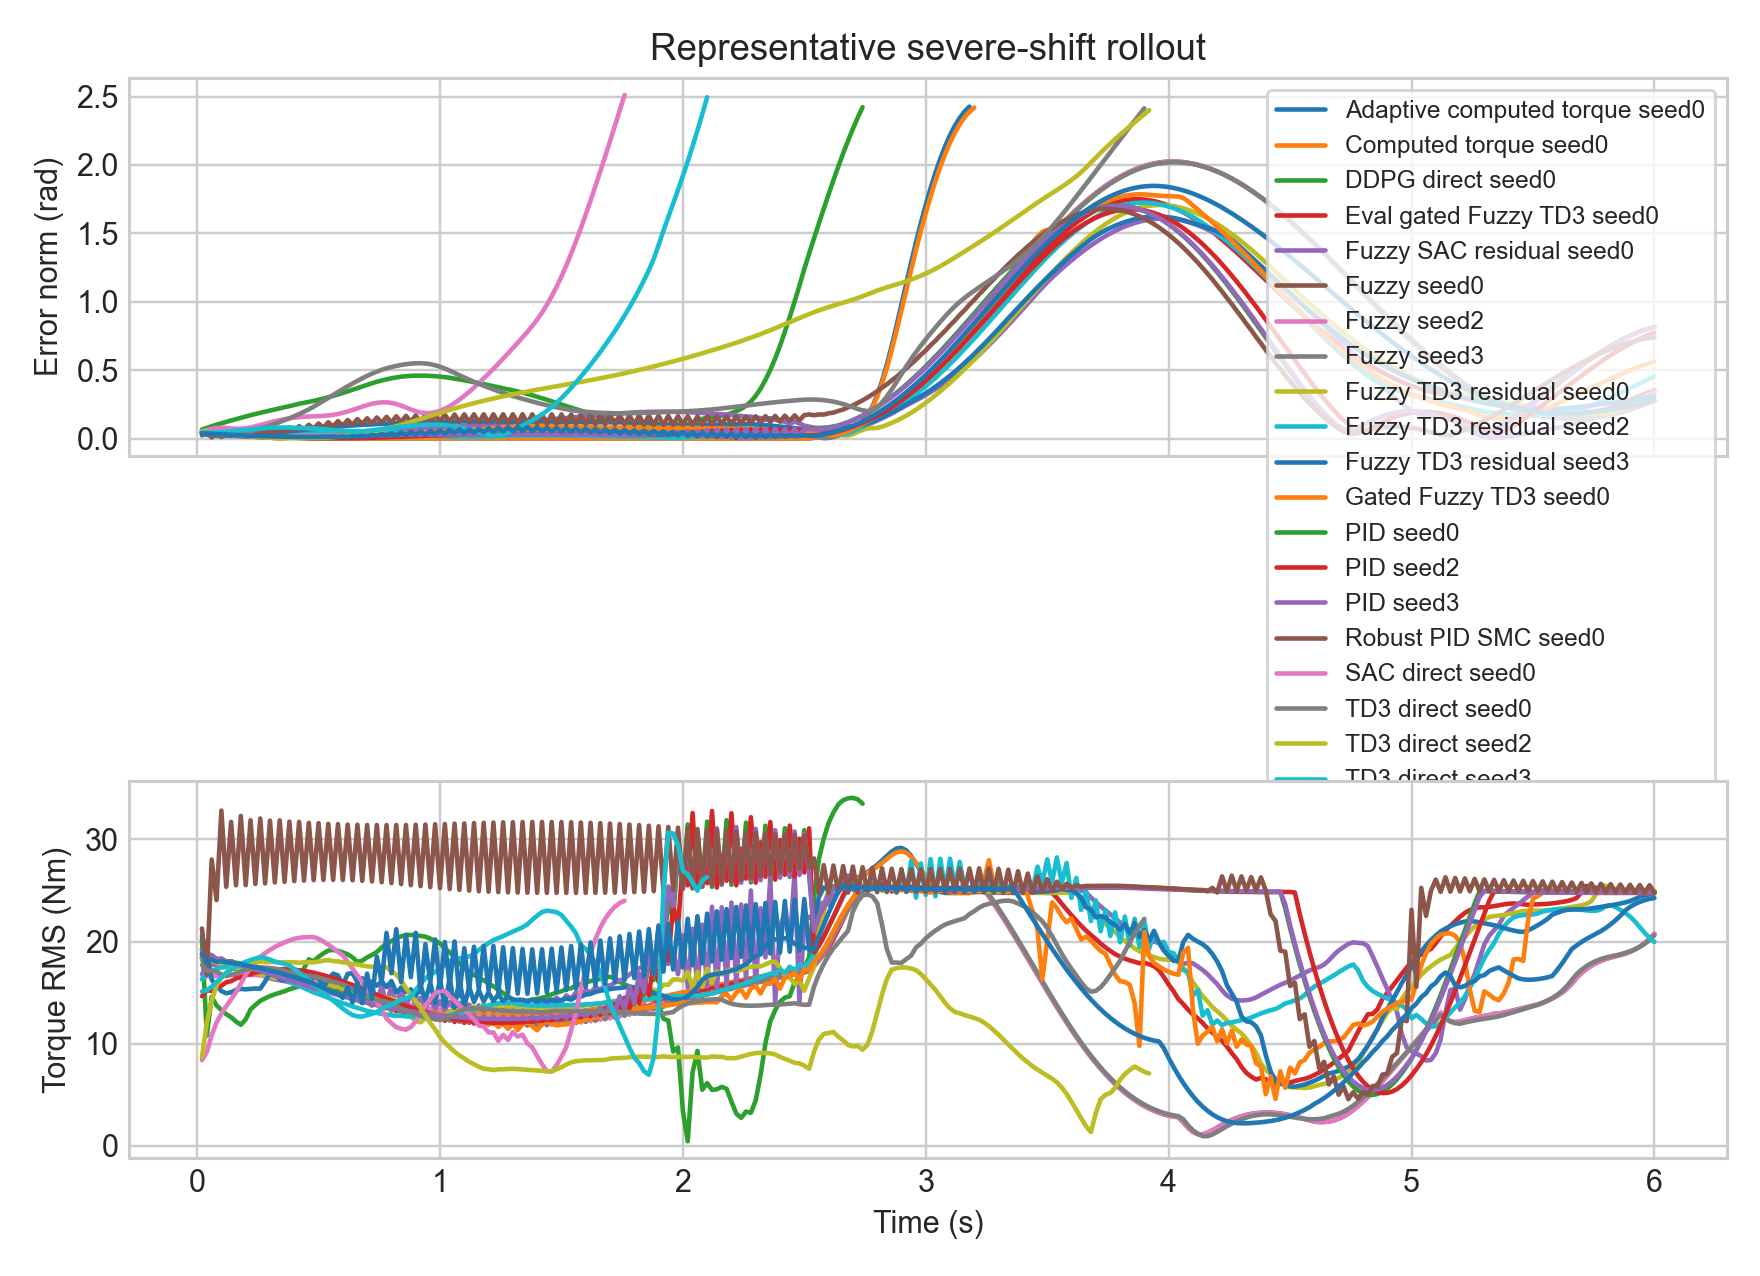
\includegraphics[width=\linewidth,height=0.78\textheight,keepaspectratio]{severe_shift_rollout.png}
  \vfill
  \small Severe-shift traces show where residual learning helps and where classical baselines remain competitive.
\end{frame}

\begin{frame}{Safety and Stability Framing}
  \begin{block}{What we can honestly claim}
    \[
      \|\bm{\tau}_{\mathrm{RL}}\|_\infty \leq \bar{\tau}_r,\quad 0\leq g\leq1
    \]
    so residual authority is explicitly bounded.
  \end{block}
  \begin{itemize}
    \item Learned residual enters the controller as a bounded additive torque.
    \item Passivity-style filtering can limit residual work against tracking-error velocity.
    \item This supports practical boundedness under standard assumptions.
  \end{itemize}
  \vfill
  \keyclaim{This is not a complete Lyapunov theorem for the neural policy. A journal version should add CBF, Lyapunov-constrained RL, or passivity-constrained policy optimization.}
\end{frame}

\begin{frame}{Limitations}
  \begin{itemize}
    \item Current validated benchmark is 2-DOF, not yet UR5/Panda/KUKA-scale.
    \item PyBullet installation failed locally because Microsoft C++ Build Tools were missing.
    \item The gate is hand-designed/evaluation-time, not yet learned or formally verified.
    \item Longer training budgets and hardware-in-the-loop latency tests are still needed.
  \end{itemize}
  \vfill
  \begin{block}{Journal-readiness status}
    Strong preliminary manuscript and reproducible benchmark; not yet a final high-impact journal submission until 6-DOF or hardware validation is completed.
  \end{block}
\end{frame}

\begin{frame}{Next Experiments Before Submission}
  \begin{enumerate}
    \item Run the same protocol on UR5, Franka Panda, KUKA iiwa, or xArm6 in PyBullet/MuJoCo/Gazebo.
    \item Replace hand-designed gate with an uncertainty estimator or learned gate.
    \item Add CBF or Lyapunov-style residual safety filter.
    \item Extend to 10 seeds and longer training horizon.
    \item Report hardware or real-time edge latency if possible.
  \end{enumerate}
  \vfill
  \keyclaim{The upgraded research idea is credible because the experiments now reveal both the benefit and the boundary of the method.}
\end{frame}

\begin{frame}{Final Takeaway}
  \begin{center}
    \Large Fuzzy-supervised residual RL is best framed as\\[0.25em]
    \textbf{an uncertainty-triggered adaptation layer}\\[0.25em]
    rather than a universal controller replacement.
  \end{center}
  \vfill
  \begin{block}{Most defensible result}
    Residual SAC/TD3 improve robustness under payload and friction shift, direct RL fails frequently, and gating preserves nominal fuzzy-control performance.
  \end{block}
  \vfill
  \begin{center}
    \large Thank you
  \end{center}
\end{frame}

\end{document}
